\documentclass[11pt,a4paper,english]{article} % document type and language

\usepackage[english]{babel}
\usepackage{tabularx}
\usepackage{cancel}
\usepackage{multirow}
\usepackage{supertabular}
\usepackage{algorithmic}
\usepackage{algorithm}
\usepackage{amsthm}
\usepackage{float}
\usepackage{subfig}
\usepackage{rotating}

\graphicspath{{../figures_supplement/}}          % graphics
\renewcommand{\thefigure}{S\arabic{figure}}
\renewcommand{\thetable}{S\arabic{table}}

\begin{document}
\clearpage
\setcounter{page}{1}
\setcounter{section}{1}
\setcounter{figure}{0}

\section*{Supplement}

\begin{figure*}[th]
  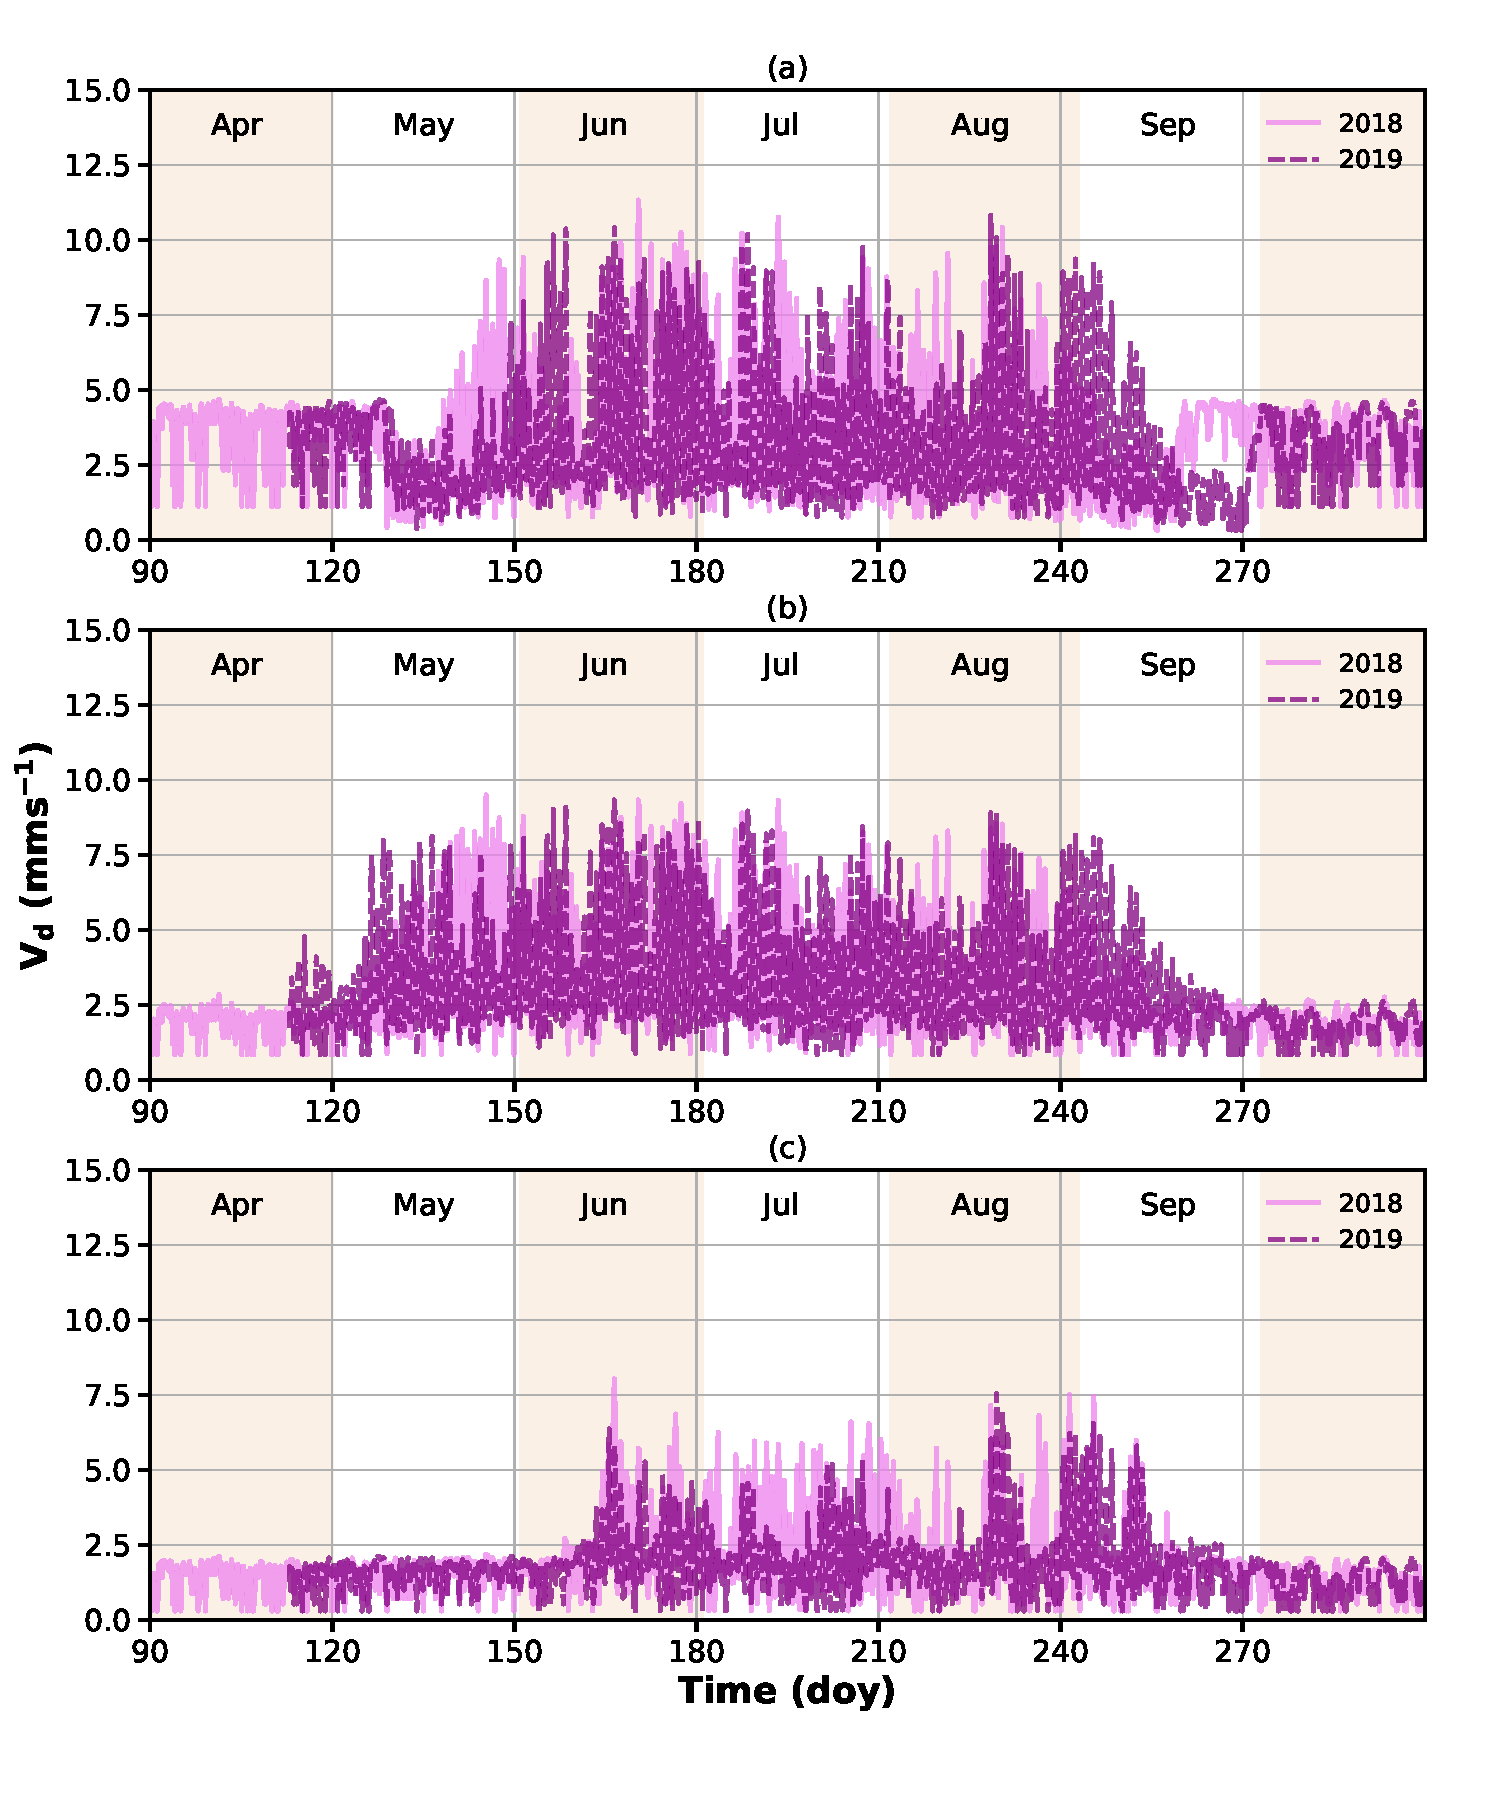
\includegraphics[width=0.95\textwidth]{DO3SE_results_Vd_MM}
  \caption{Time series of $\mathrm{DO_3SE}$ modeled ozone dry deposition velocities for mapping manual temperature and light response functions in GS 2018/19. (a) Deciduous trees; (b) coniferous trees; (c) perennial grassland.}
  \label{fig:dose_results_vd_mm}
\end{figure*}

\begin{figure*}[th]
  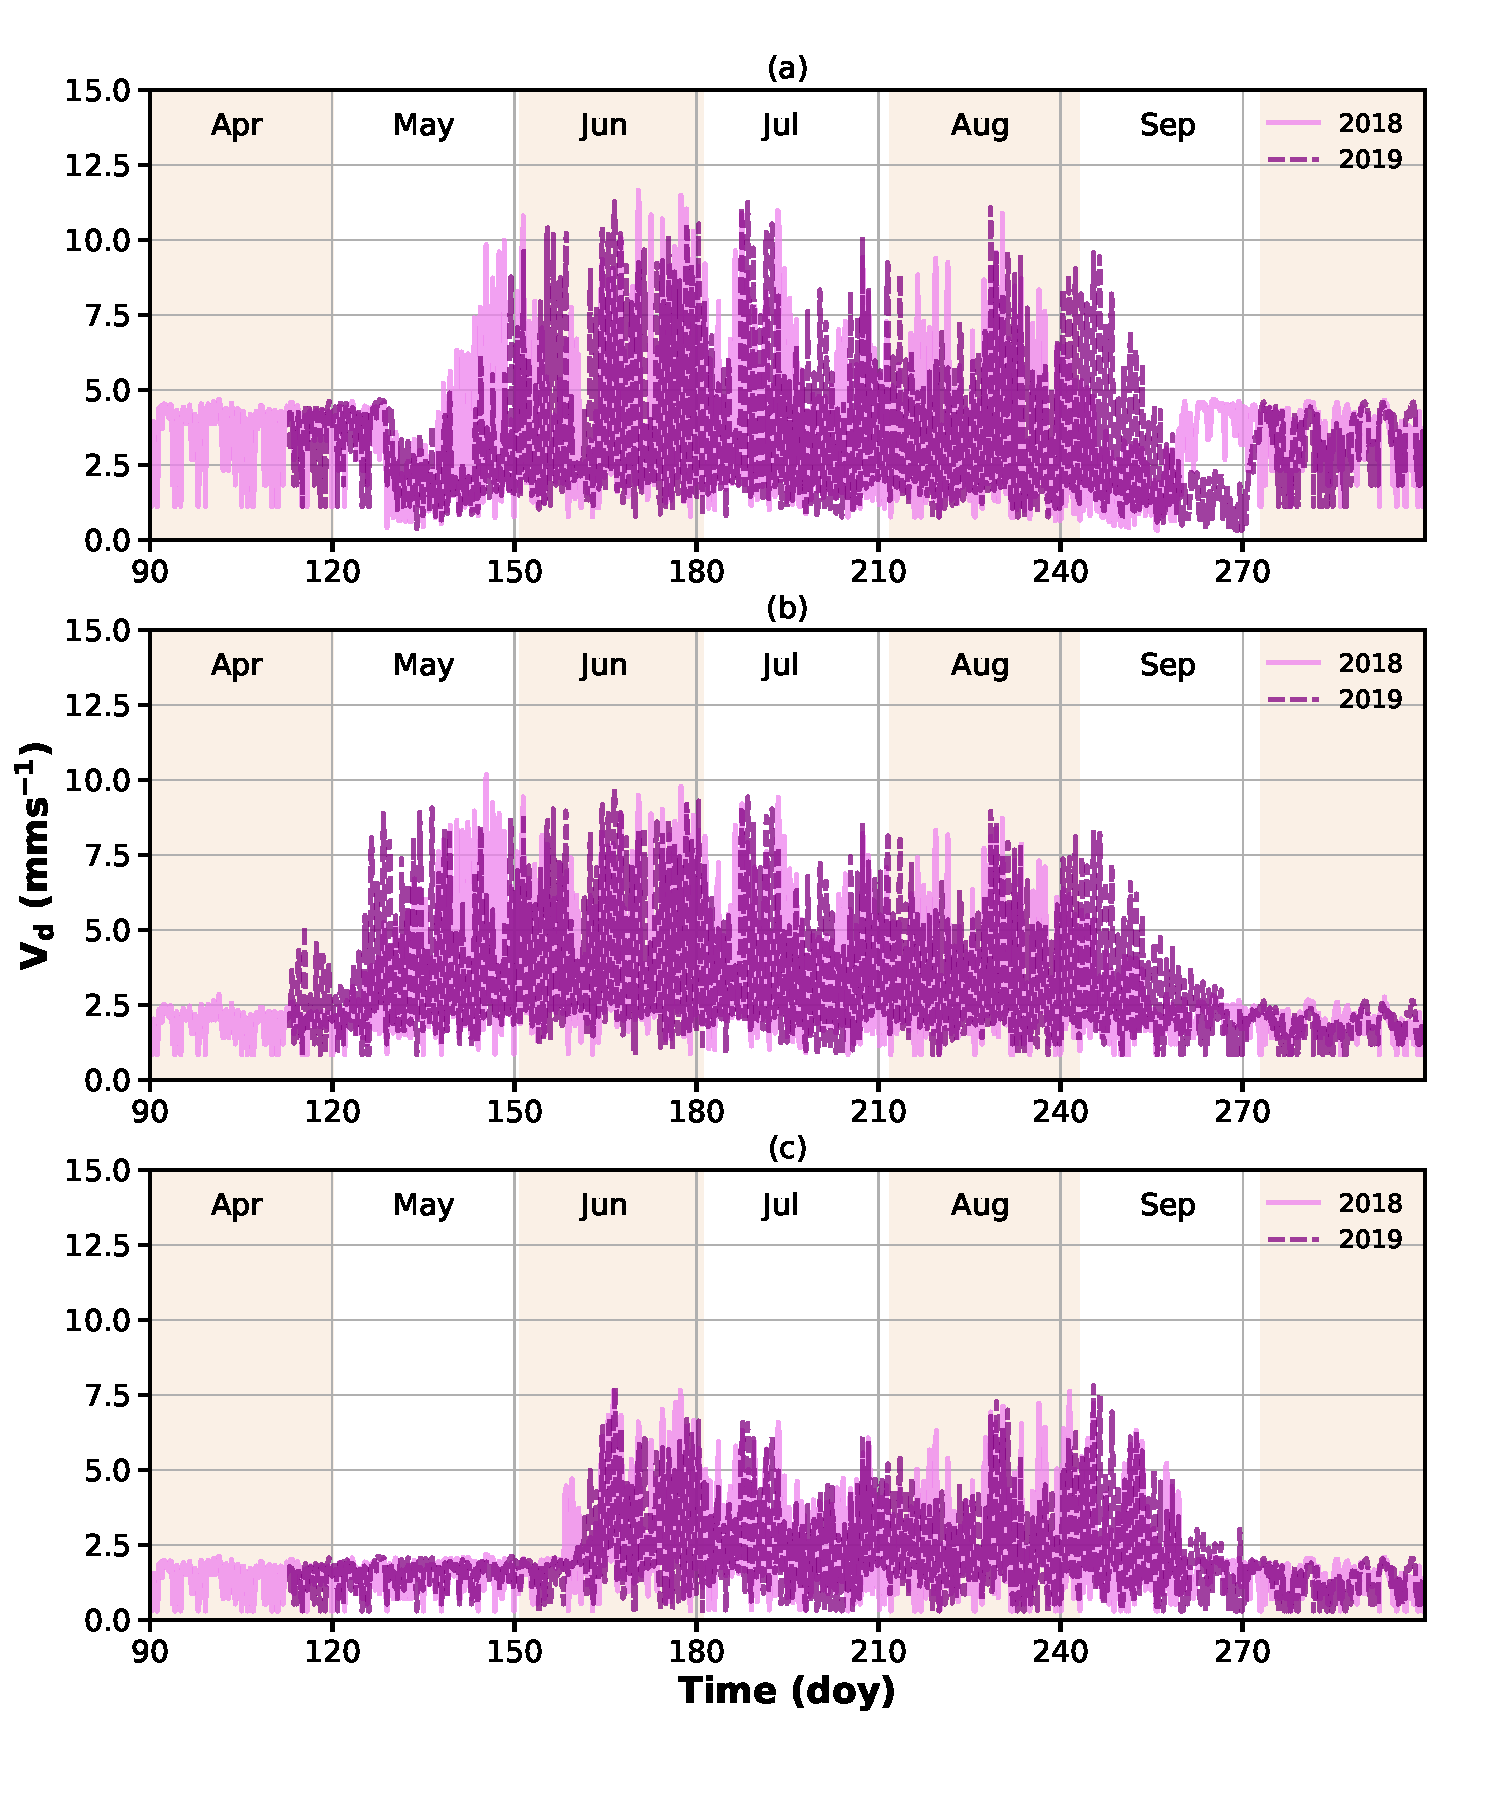
\includegraphics[width=0.95\textwidth]{DO3SE_results_Vd_Cold}
  \caption{Time series of $\mathrm{DO_3SE}$ modeled ozone dry deposition velocities for "cold" temperature and light response functions in GS 2018/19. (a) Deciduous trees; (b) coniferous trees; (c) perennial grassland.}
  \label{fig:dose_results_vd_cold}
\end{figure*}

\begin{figure*}[th]
  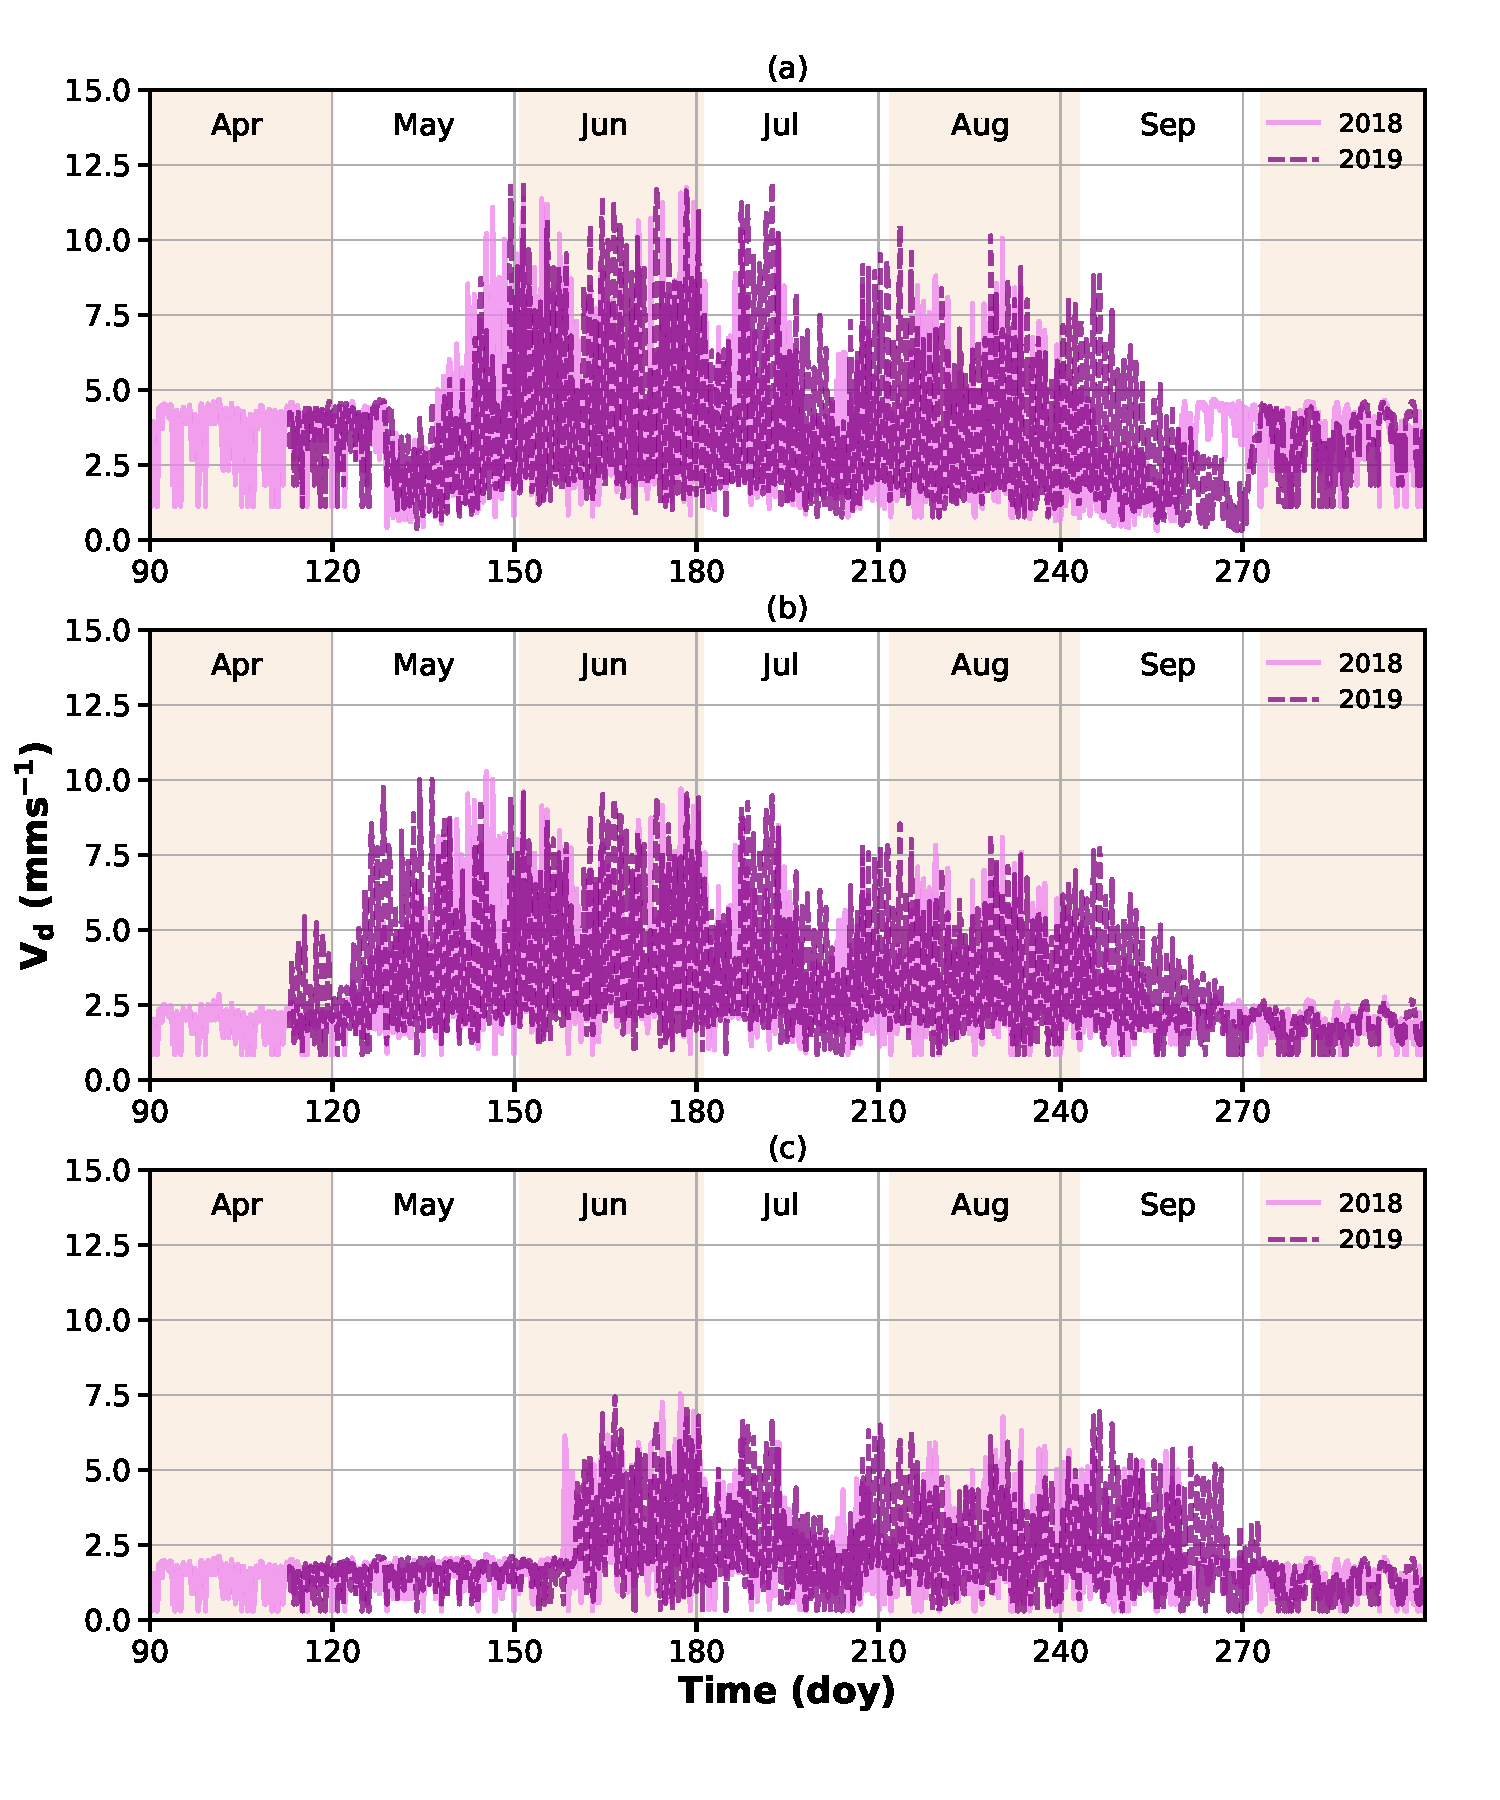
\includegraphics[width=0.95\textwidth]{DO3SE_results_Vd_Boreal}
  \caption{Time series of $\mathrm{DO_3SE}$ modeled ozone dry deposition velocities for "subarctic" temperature and light response functions in GS 2018/19. (a) Deciduous trees; (b) coniferous trees; (c) perennial grassland.}
  \label{fig:dose_results_vd_subarctic}
\end{figure*}

\begin{figure*}[th]
  \hspace*{-3cm}
  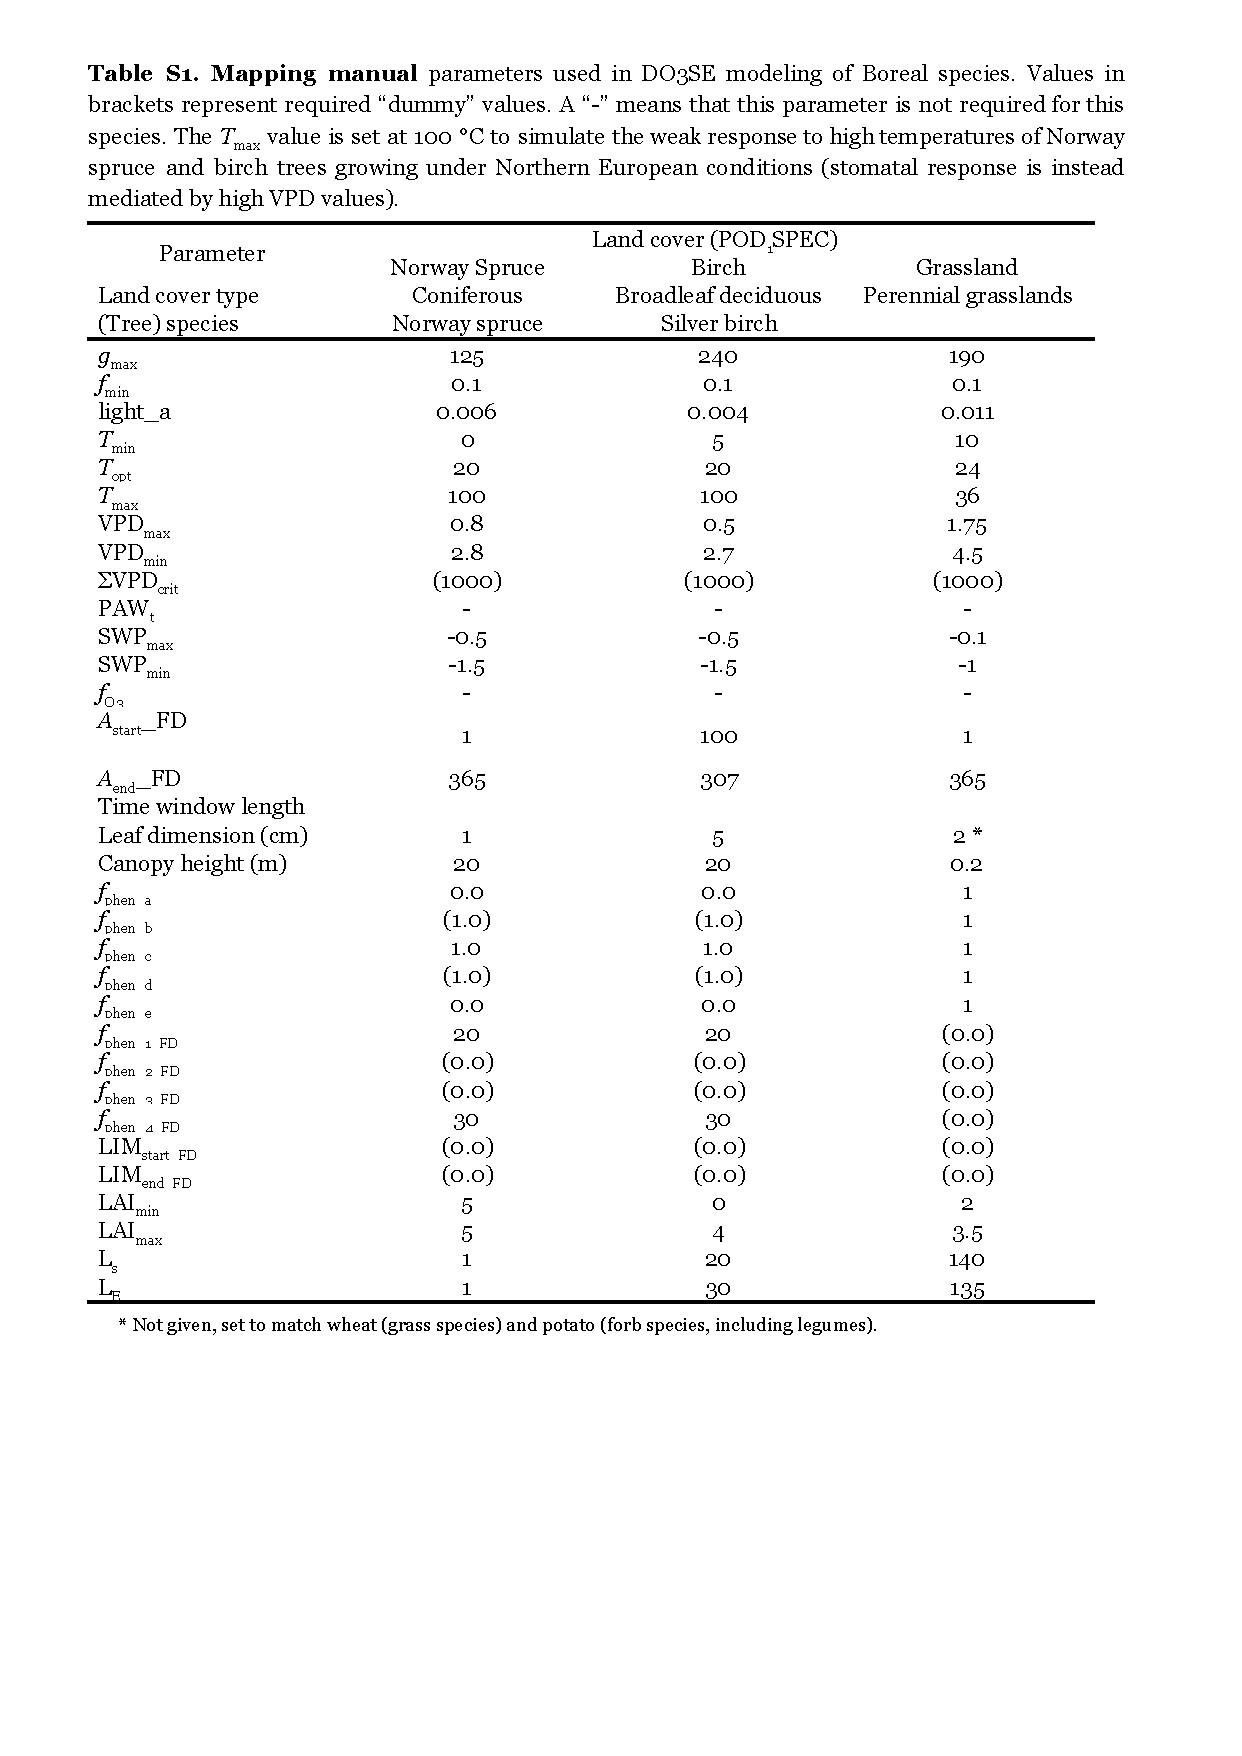
\includegraphics[width=1.5\textwidth]{supplement_do3se-parameterization_v2}
  \label{tab:do3se_mm_param}
\end{figure*}

\end{document}